\chapter{Experimentos y resultados}\label{chapter:results}

En este capítulo se presentan los experimentos realizados para evaluar el desempeño y los resultados de la regresión simbólica propuesta en este trabajo.

En la sección \ref{section:experimental_considerations} se menciona como se diseñó el marco experimental para realizar distintos experimentos. En \ref{section:experimental_frame} se plantea la forma en la que se generaron los datos utilizados en los distintos experimentos y cómo se modeló la presencia de ruido en las muestras. En la sección \ref{section:experiments} se desarrollan los experimentos realizados y se aprecian sus resultados. En \ref{section:experiments_results} se analizan los resultados obtenido. A continuación se describen detalles acerca del diseño del marco experimental que se utilizó en la realización de los experimentos.

\section{Consideraciones de la etapa de experimentación}\label{section:experimental_considerations}

El espacio de búsqueda en la regresión simbólica que se propone en este trabajo comprende a todos los sistemas de ecuaciones diferenciales lineales con respecto a los parámetros donde la cantidad de ecuaciones se define según los datos. La regresión simbólica es un problema NP-difícil por lo que resulta computacionalmente costoso. Para lidiar con este costo computacional se diseñó un marco experimental que fuese factible de ejecutar en un ordenador portátil. El equipo de cómputo donde se realizaron los experimentos posee las siguientes propiedades.

\begin{itemize}
    \item \textbf{Procesador}: 11th Gen intel i9-11900H @ 2.50GHz
    \item \textbf{RAM}: 40GB
    \item \textbf{Arquitectura}: 64 bits
\end{itemize}

La implementación de la solución se desarrolla en el lenguaje de programación \emph{Python} auxiliado por bibliotecas como \emph{numpy} \cite{harris2020array} y \emph{scipy} \cite{2020SciPy-NMeth}.

Como métrica para evaluar la calidad de la solución generada por la regresión simbólica se utiliza el error cuadrático medio. Menores valores de esta métrica implica que el valor de los datos evaluados en el sistema obtenido en la regresión simbólica se acercan a los datos observados.

Cada experimento que aparece en la sección \ref{section:experiments} se realizó 30 veces y se plantea el valor promedio que obtuvo la métrica utilizada en las 30 ejecuciones del experimento. Además se indica el valor mínimo y máximo que alcanzó la métrica a lo largo de los 30 experimentos. De igual forma se plantea cuántas veces en la realización de los 30 experimentos, el método de regresión simbólica encuentró un sistema igual al tomado para generar los datos.

En la siguiente sección se precisa mejor cómo se generan los datos para realizar los distintos experimentos.

\section{Descripción del marco experimental}\label{section:experimental_frame}

Los experimentos inician con la selección de un modelo conocido $f$, por ejemplo el modelo SIR:

\begin{align*}
    S' & = - aIS    \\
    I' & = aIS - bI \\
    R' & = bI.
\end{align*}

El sistema de ecuaciones diferenciales se integra en un intervalo que se define mediante parámetros y se obtiene un conjunto de puntos que representan el valor de las distintas variables a lo largo del tiempo. Por ejemplo, si se integra el modelo SIR utilizando como parámetros $a = 0.0003$, $b = 0.1$ y con $0 \leq t \leq 20$ se obtienen las curvas en la imagen \ref{fig:SIR}.

\begin{figure}[h]
    \centering
    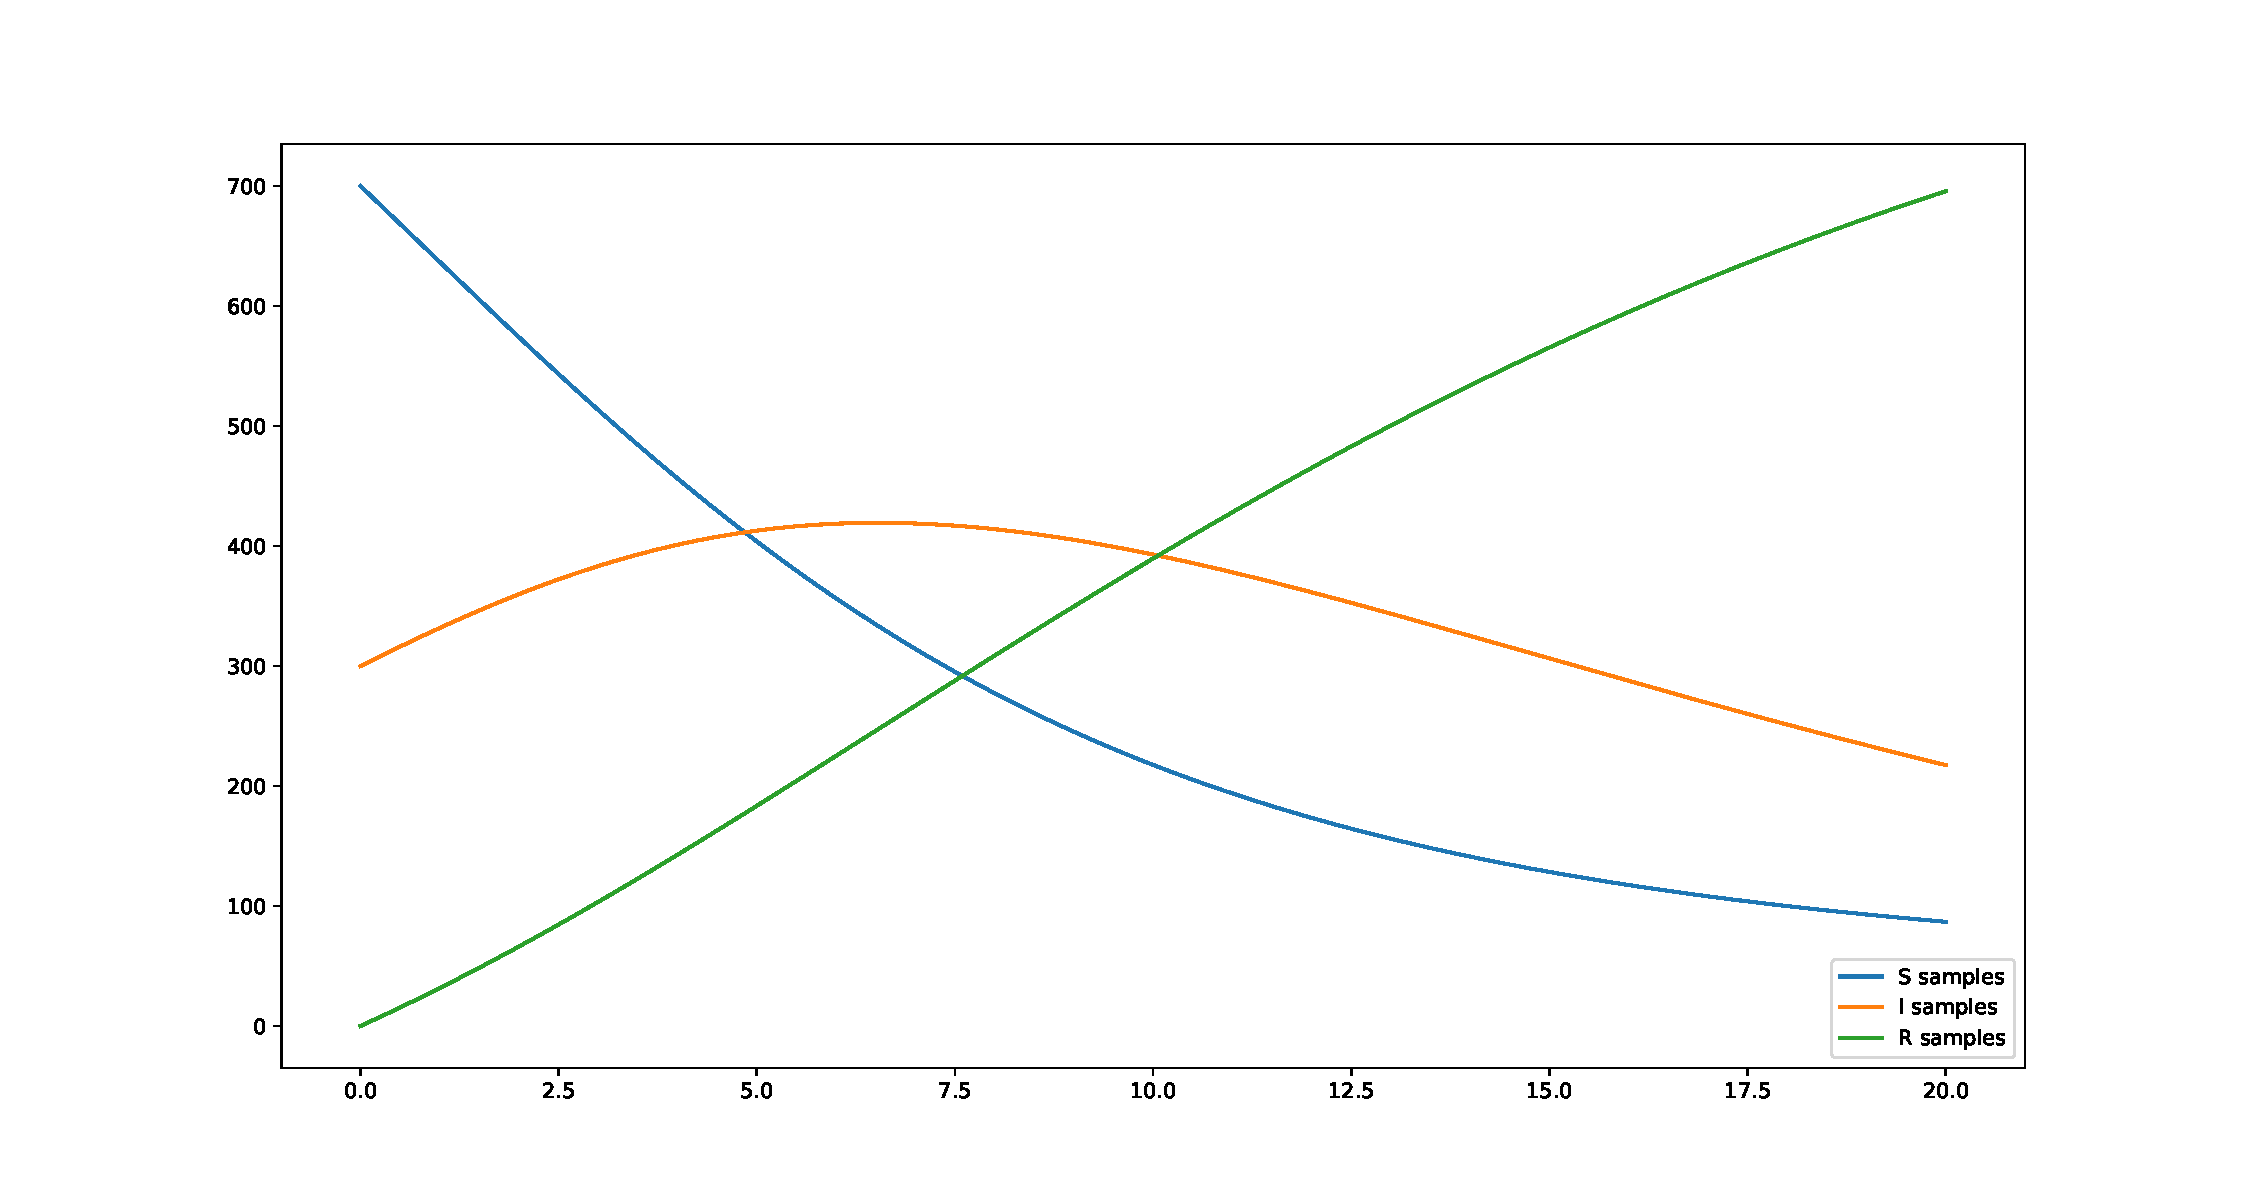
\includegraphics[width=\textwidth]{"figures/SIR.pdf"}
    \caption{modelo SIR con $a = 0.0003$, $b = 0.1$.}
    \label{fig:SIR}
\end{figure}

Luego de que se tienen los datos de la forma $\{(t_i, y_i)\}$ generados por la integración del modelo, se le agregan distintos valores de ruido a los puntos. A cada muestra $y_i$ se le agrega un valor de ruido utilizando la fórmula:

$$y_{i_{noise}} = y_i + y_i * max\_noise * random\_standard\_normal(),$$

donde $random\_standard\_normal()$ es una función que genera valores aleatorios, independientes y con media 0. $max\_noise$ es un parámetro con mínimo valor $0$ y máximo $1$ que define el ``ruido  máximo'' que se le agrega a cada muestra. Se puede ver el parámetro $max\_noise$ como el \% máximo del valor de cada muestra que se puede agregar como ruido. Durante los distintos experimentos se utilizaron como máximo ruido los valores de 0\%, 5\% o 10\% con respecto a cada muestra. Por ejemplo, si se agrega ruido a los datos obtenidos de la integración del sistema SIR utilizando el parámetro $max\_noise$ con valor $0.1$, se tendrían las curvas que aparecen en la imagen \ref{fig:SIR_with_noise}.

\begin{figure}[h]
    \centering
    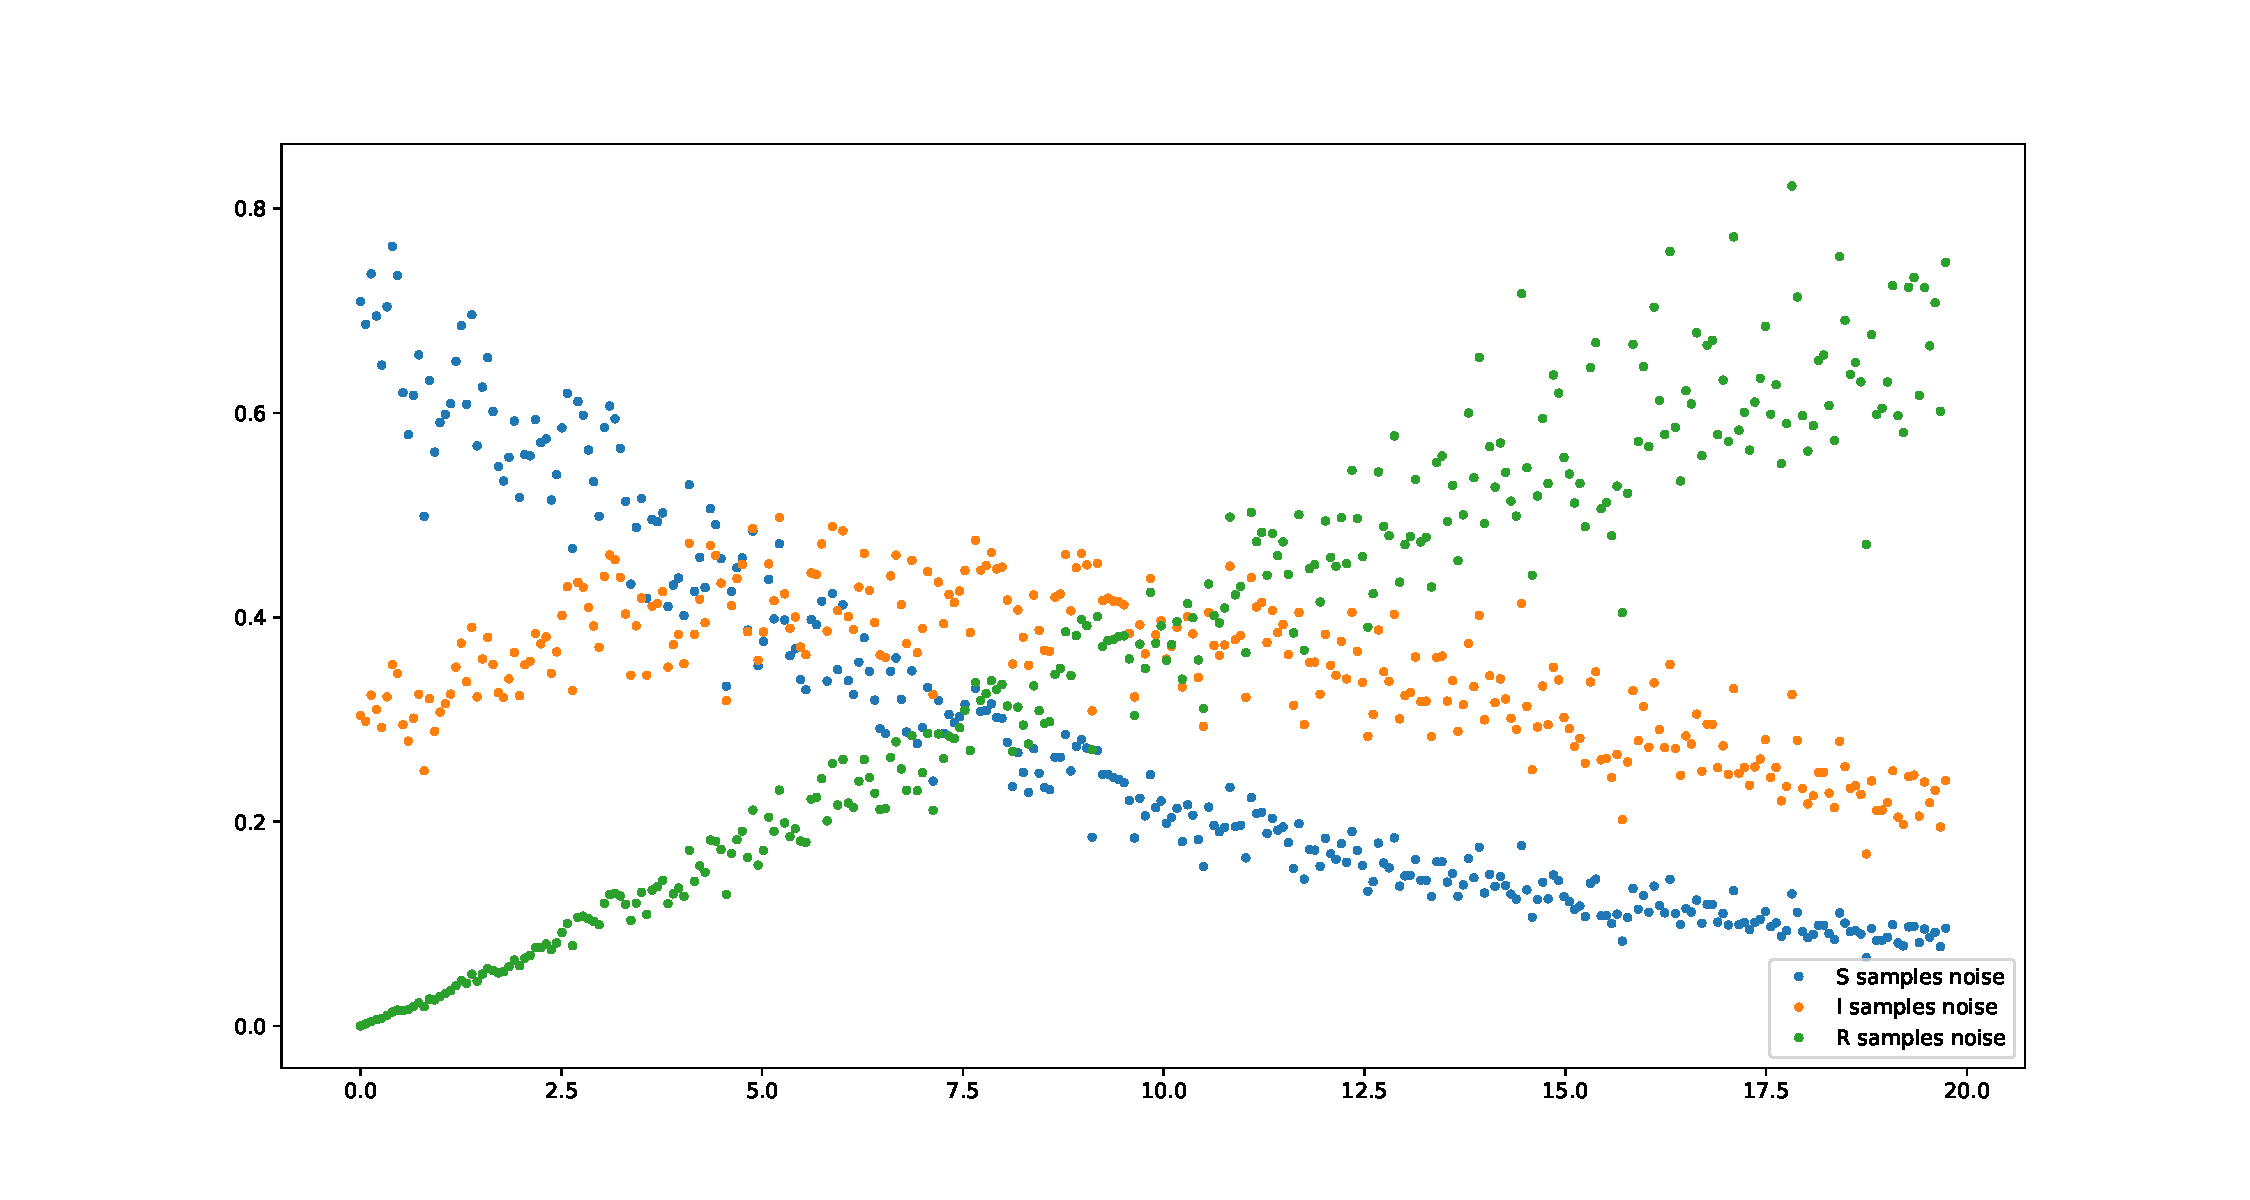
\includegraphics[width=\textwidth]{"figures/SIR_with_noise.pdf"}
    \caption{modelo SIR con $a = 0.0003$, $b = 0.1$ y $max\_noise = 0.1$.}
    \label{fig:SIR_with_noise}
\end{figure}

Se utiliza un spline de suavizado para eliminar el ruido en caso de que $max\_noise > 0$. El valor del parémtro de suavizado en el spline se varía para cada una de las variables. Por ejemplo, si se utiliza un spline de suavizado cúbico en los datos con ruido del sistema SIR se obtendrían las curvas que aparecen en la imagen \ref{fig:SIR_noise_with_spline}.

\begin{figure}[h]
    \centering
    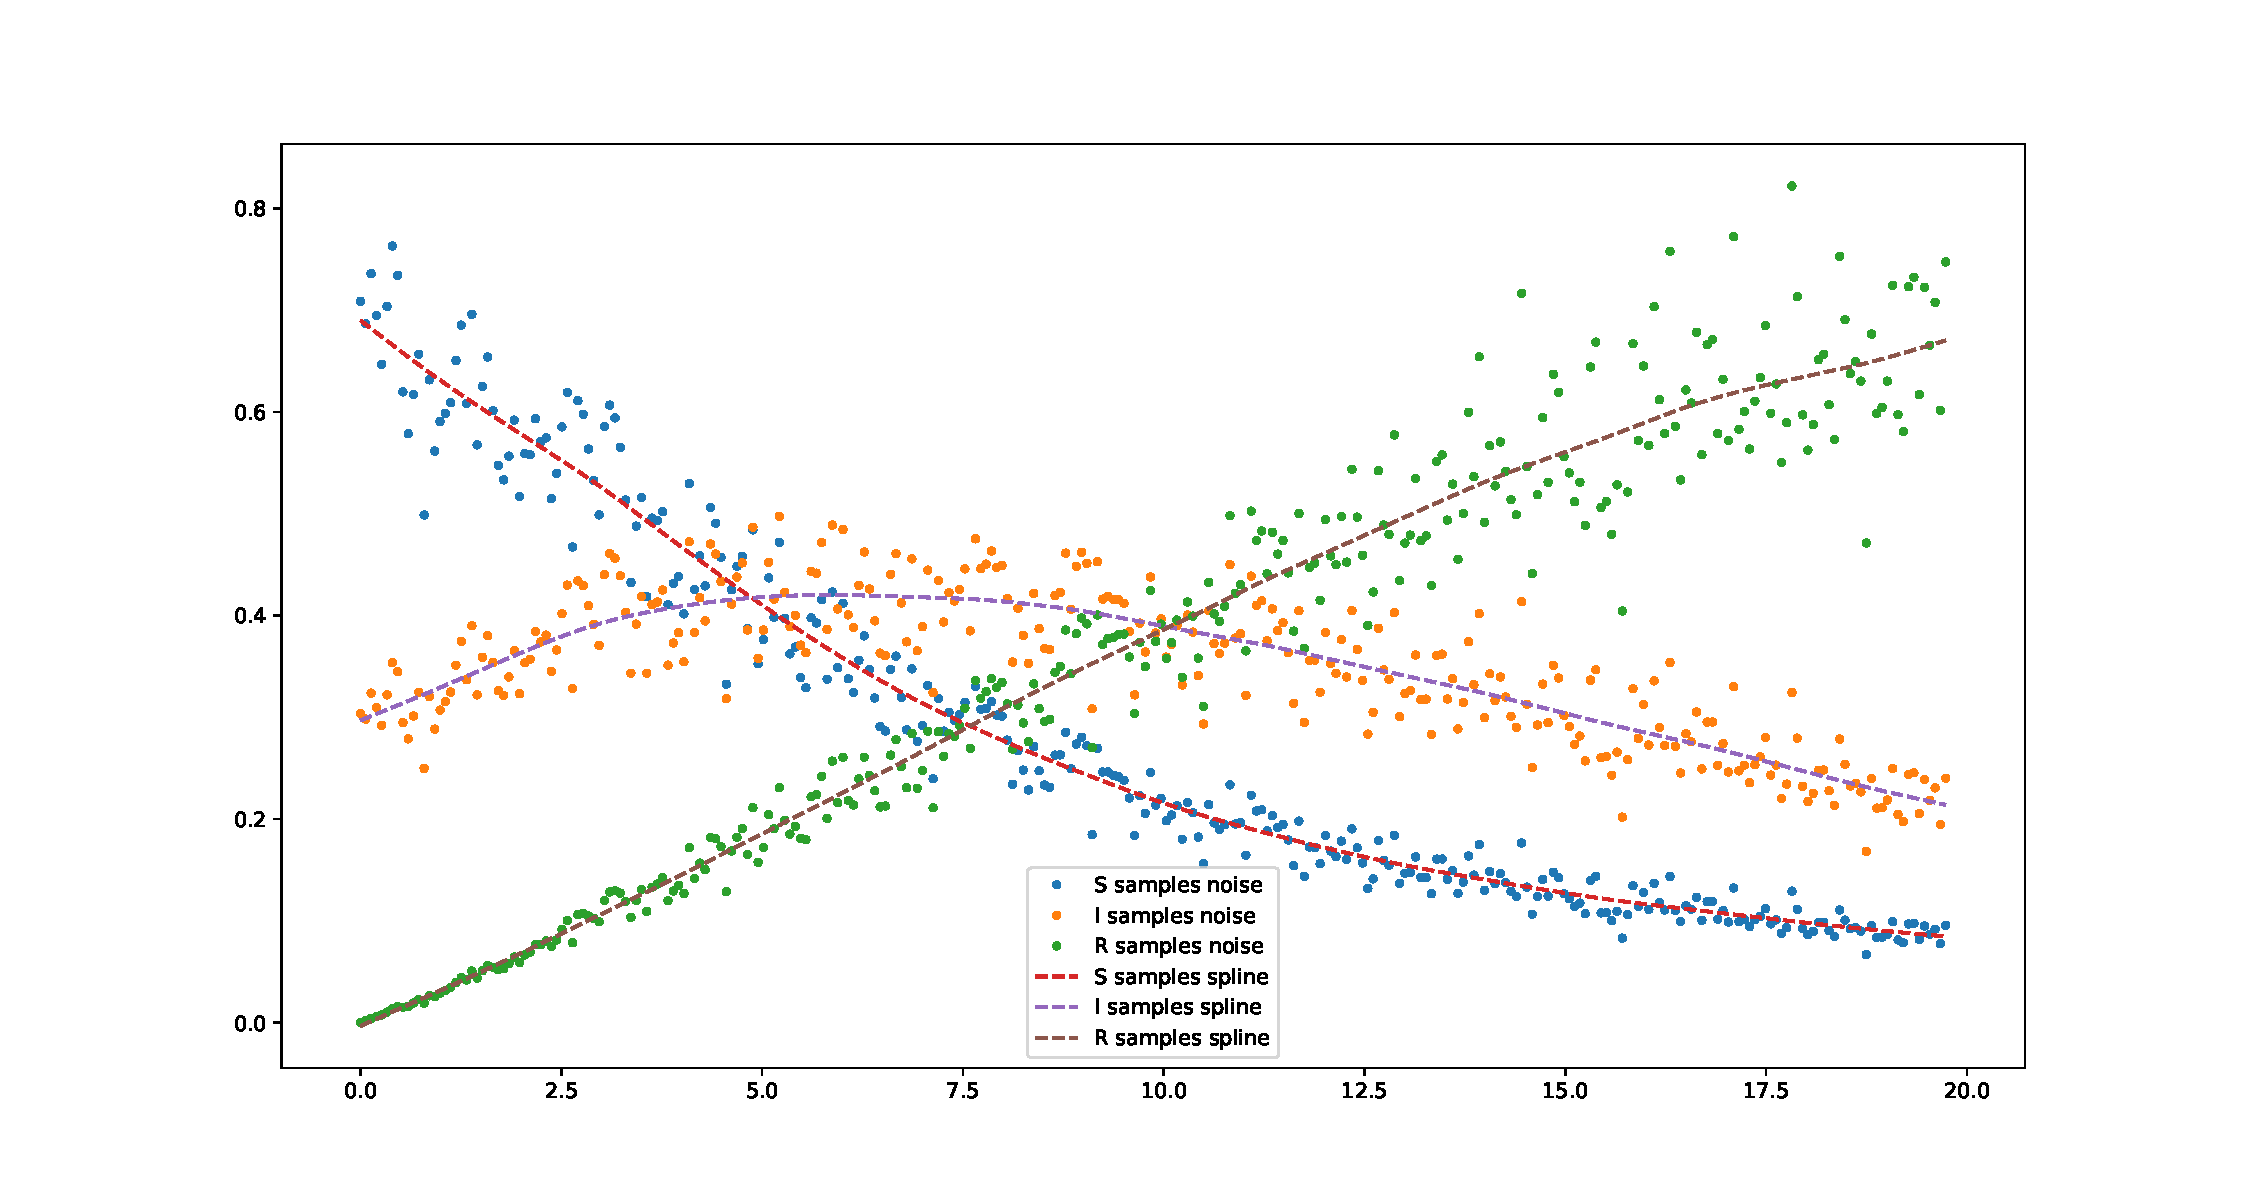
\includegraphics[width=\textwidth]{"figures/SIR_noise_with_spline.pdf"}
    \caption{modelo SIR con $a = 0.0003$, $b = 0.1$, $max\_noise = 0.1$ y smoothing-spline con valor de suavizado de $0.1$.}
    \label{fig:SIR_noise_with_spline}
\end{figure}

Una vez que se tiene el spline de suavizado, se puede aproximar el valor de la función $y$ que describen los datos que se generaron mediante la integración de un modelo $f$. Junto a la aproximación de la función se puede obtener la primera derivada del spline de suavizado. La derivada permite obtener una aproximación del valor de $f$.

Se pueden utilizar la aproximación de la función $y$ y las aproximaciones de $f$ mediante las derivadas del spline de suavizado para encontrar el sistema de ecuaciones diferenciales mediante el uso de la regresión simbólica.

Se presentan en las siguientes secciones los experimento en los que se utliza la regresión simbólica para encontrar el sistema de ecuaciones diferenciales lineales con respecto a los parámetros a partir de un conjunto de datos generado. Se utilizaron en total 5 modelos para la generación de los disintos conjuntos de datos.

\section{Experimentos realizados}\label{section:experiments}

Todos los sistemas de ecuaciones diferenciales seleccionados son sistemas lineales en los parámetros. La cantidad de ecuaciones en cada uno de los modelos es distinta. De cada modelo seleccionado se muesta una tabla que contiene la media del valor de la función de ajuste a lo largo de las 30 ejecuciones del experimento así como el mínimo y máximo valor que alcanzó el error cuadrático medio.

En otra tabla se detalla la media del error cuádratico medio entre los datos $y_{sr}$ generados por la integración del sistema encontrado en la regresión simbólica y datos utilizados durante el método de regresión simbólica. Esta media del error cuadrático media es sobre una cantidad de experimentos tomados de los 30 experimentos realizados, la cantidad de experimentos seleccionados se define en la fila ``cantidad de experimentos''. La diferencia de $y_{sr}$ con respecto $y_{original}$ a los generados por la integración del sistema original del experimento aparecen en la fila llamada ``orignal''. En la fila ``original con ruido'' aparece el error cuadrático medio de $y_{sr}$ y los datos $y_{noise}$ que se generan al agregar ruido al conjunto $y_{original}$, El ruido máximo agregado se define en las columnas de la tabla. La diferencia de $y_{sr}$ con respecto a los datos obtenidos a partir del spline de suavizado generado por los datos $y_{noise}$ se encuentra en la fila ``spline''. Como última fila en la tabla se muestra el error cuádratico medio entre los datos $y_{original}$ evaluados en el sistema obtenido en la regresión simbólica y los datos $y_{original}$ evaluados en el sistema obtenido utilizando otro método[LE TENGO QUE PREGUNTAR A OLIVIA CUÁL MÉTODO USÓ].

A continuación se muestra el experimento realizado a partir de la generación de los datos utlizando el sistema Lotka-Volterra.

\subsection{Lotka-Volterra}

El modelo de Lotka-Volterra es un sistema utilizado para describir las interacciones entre dos especies, una como depredador y otra como presa \cite{Hoppensteadt:2006}. La población de cada especie cambia a través del tiempo de acuerdo al sistema de ecuaciones diferenciales:

\begin{align*}
    X' & = X (a - b Y)   \\
    Y' & = -Y (c - d X).
\end{align*}

Se utilizaron como valores de los parámetros $a = 0.04$, $b = 0.0005$, $c = 0.2$ y $d = 0.004$ con punto inicial $(20, 20)$ y se integró en el intervalo $0 \leq t \leq 300$ para obtener los datos que aparecen en la figura \ref{fig:lotka_volterra}. Del conjunto de puntos se seleccionaron 300 muestras como datos para el método de regresión simbólica.

\begin{figure}[h]
    \centering
    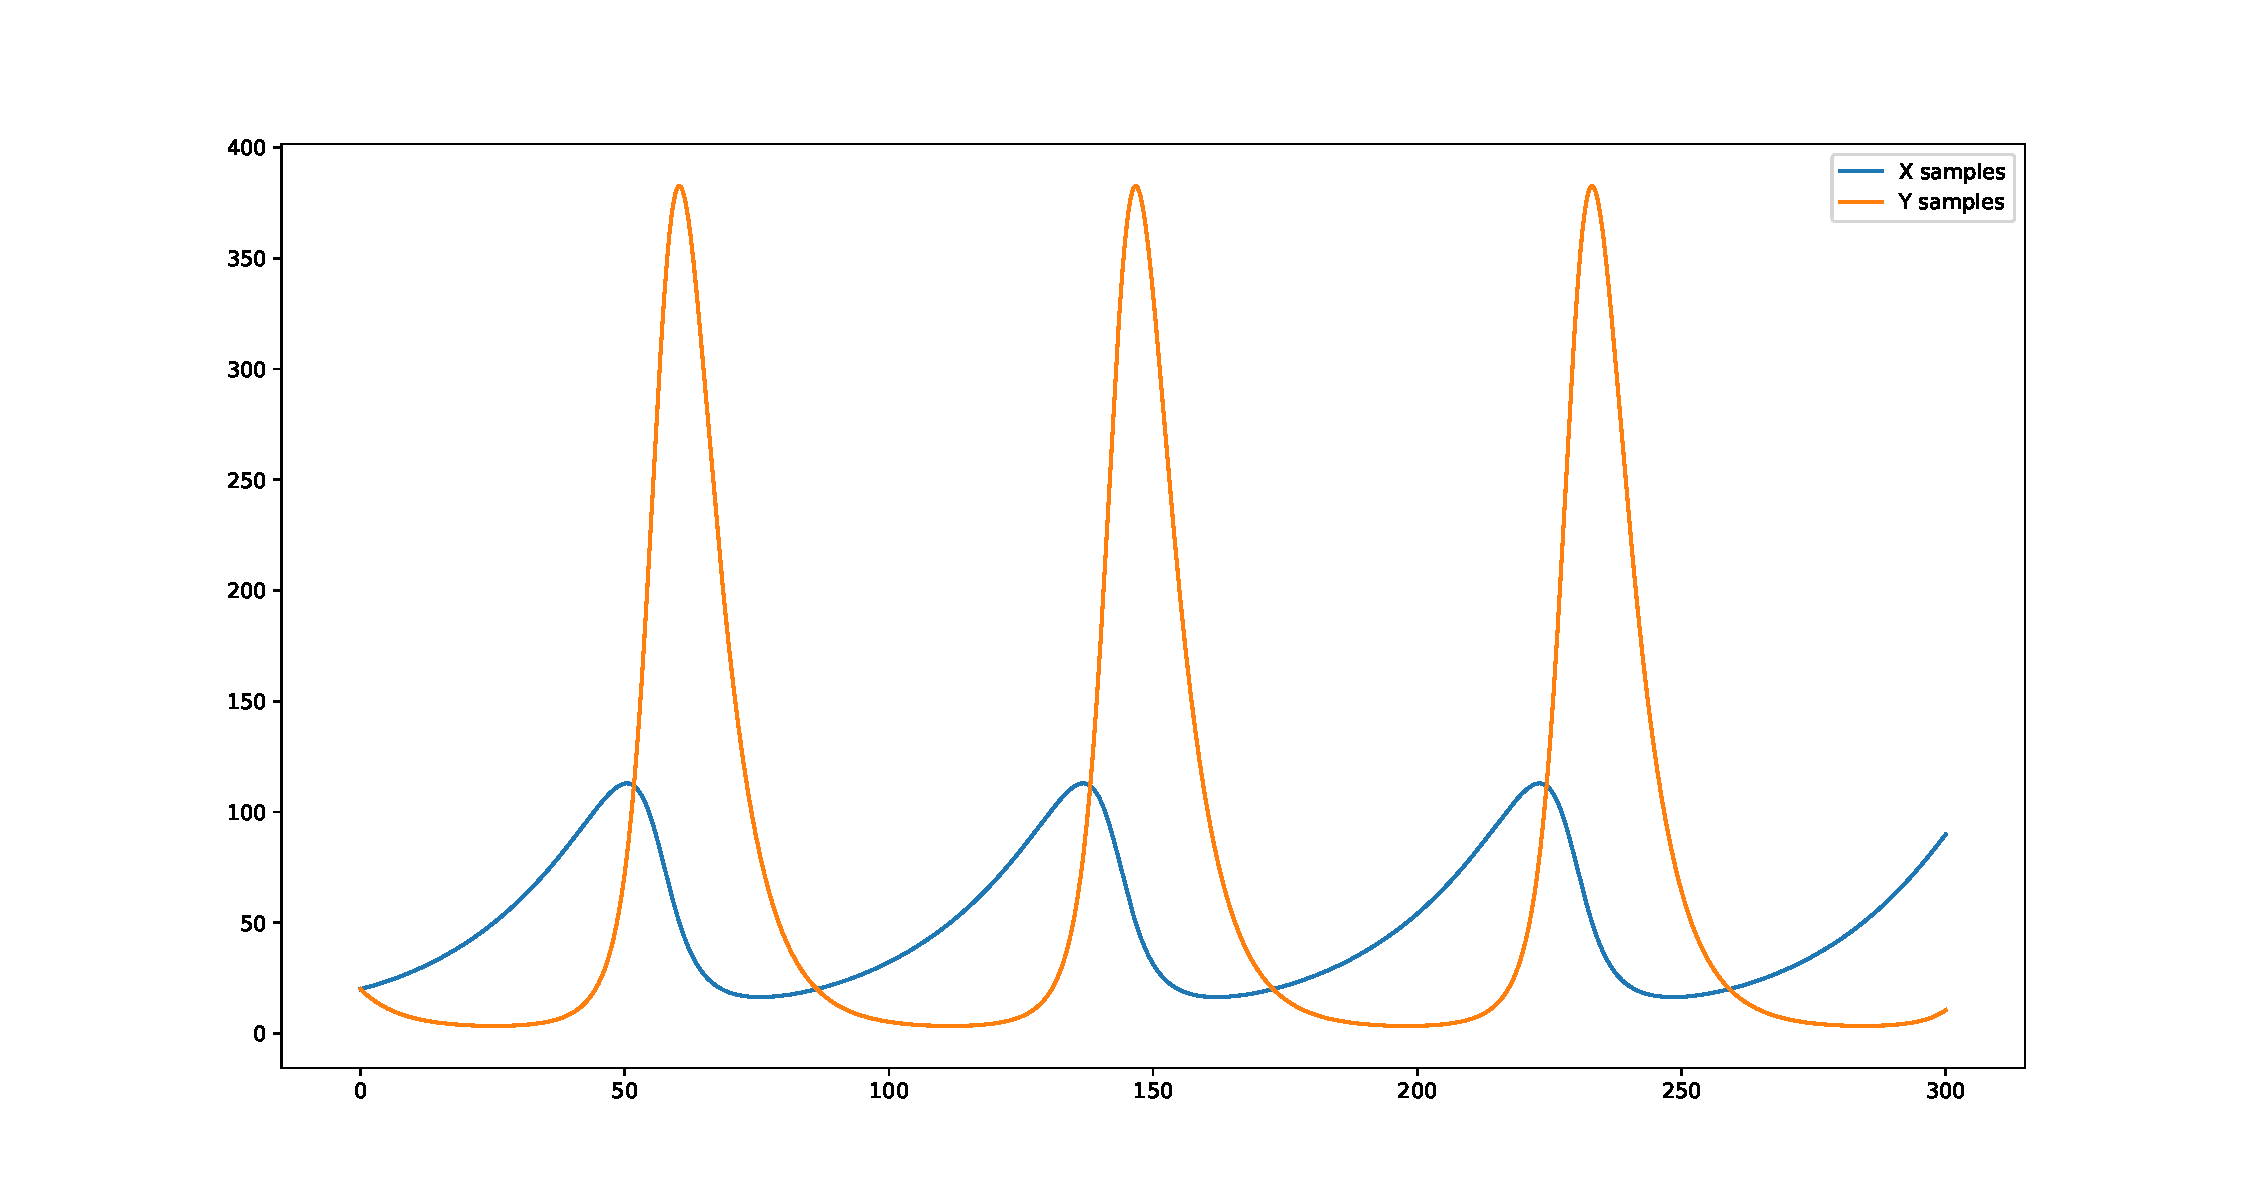
\includegraphics[width=\textwidth]{"figures/lotka_volterra.pdf"}
    \caption{modelo Lotka Volterra con $a = 0.04$, $b = 0.0005$, $c = 0.2$ y $d = 0.004$.}
    \label{fig:lotka_volterra}
\end{figure}

Los resultados que se obtienen durante las 30 ejecuciones del experimento aparecen en la tablas \ref{table:experiment_lotka_volterra}.

\begin{table}[!h]
    \centering
    \caption{Resultados obtenidos en el modelo Lotka-Volterra}

    \begin{tabular}{|c|c|c|c|}
        \hline
               & \textbf{ruido de 0\%} & \textbf{ruido de 5\%} & \textbf{ruido de 10\%} \\
        \hline
        media  & 0.74514               & 0.69138               & 0.84485                \\
        \hline
        mínimo & 0.28343               & 0.42189               & 0.54373                \\
        \hline
        máximo & 0.97944               & 1.11027               & 1.68603                \\
        \hline
    \end{tabular}

    \begin{tabular}{|c|c|c|c|c|c|}
        \hline
                             & \textbf{ruido de 0\%} & \textbf{ruido de 5\%} & \textbf{ruido de 10\%} \\
        \hline
        cantidad de sistemas & 30                    & 28                    & 25                     \\
        \hline
        original             & 17.01575              & 52.17101              & 50.30572               \\
        \hline
        original con ruido   & 17.01575              & 52.21558              & 50.56727               \\
        \hline
        spline               & 17.01575              & 51.85661              & 49.99422               \\
        \hline
        otro método          & 1394.26981            & 1111.95166            & 1519.66141             \\
        \hline
    \end{tabular}

    \label{table:experiment_lotka_volterra}
\end{table}

A continuación se muestra el experimento realizado a partir de la generación de los datos utilizando el sistema SIR.

\subsection{SIR}

El modelo SIR es un sistema que se utiliza para describir la transmición de una enfermedad infecciosa causada por una bacteria, virus u hongos. \cite{weiss2013sir}. Se define el sistema como:

\begin{align*}
    S' & = - aIS    \\
    I' & = aIS - bI \\
    R' & = bI,
\end{align*}

donde $S$ indica la cantidad de personas susceptibles, $I$ la cantidad de personas infectadas y $R$ la cantidad de personas recuperadas. Se utiliza el parámetro $a$ para indicar el índice de transmición y $b$ la índice de recuperación de la enfermedad.

Se utilizaron como valores de los parámetros $a = 0.0003$ y $b = 0.1$ con punto inicial $(700, 300, 0)$ y se integró en el intervalo $0 \leq t \leq 20$ para obtener los datos que aparecen en la imagen \ref{fig:SIR}. Del conjunto de puntos se seleccionaron 300 muestras como datos para el método de regresión simbólica.

Los resultados que se obtienen durante las 30 ejecuciones del experimento aparecen en la tabla \ref{table:experiment_SIR}.

\begin{table}[!h]
    \centering
    \caption{Resultados obtenidos en el modelo SIR}
    \begin{tabular}{|c|c|c|c|}
        \hline
               & \textbf{ruido de 0\%} & \textbf{ruido de 5\%} & \textbf{ruido de 10\%} \\
        \hline
        media  & 0.25506               & 4.78621               & 6.9987                 \\
        \hline
        mínimo & 0.2187                & 0.79521               & 1.48455                \\
        \hline
        máximo & 0.30485               & 31.77664              & 51.66934               \\
        \hline
    \end{tabular}

    \begin{tabular}{|c|c|c|c|c|c|}
        \hline
                             & \textbf{ruido de 0\%} & \textbf{ruido de 5\%} & \textbf{ruido de 10\%} \\
        \hline
        cantidad de sistemas & 30                    & 28                    & 28                     \\
        \hline
        original             & 2.02689               & 60.79755              & 117.71809              \\
        \hline
        original con ruido   & 2.02689               & 66.59004              & 130.68564              \\
        \hline
        spline               & 2.02689               & 61.046                & 117.83595              \\
        \hline
        otro método          & 31160.12619           & 27363.87727           & 35775.36901            \\
        \hline
    \end{tabular}
    \label{table:experiment_SIR}
\end{table}

Con este experimento se obtiene que los datos evaluados en el sistema generado por la regresión simbólica se acercan a los datos utilizados para la generación del sistema obtenido en la regresión simbólica no importa la cantidad de ruido utilizado. Los datos que se obtienen de la integración del sistema resulante de la regresión simbólica se asemejan a los datos de la integración del sistema seleccionado para la realización del experimento pero la aparición de ruido afecta el ajuste de los datos.

A continuación se muestra el experimento realizado a partir de la generación de datos utilizando el sistema SIRD.

\subsection{SIRD}

El modelo SIRD es un sistema similar al SIR pero que introduce como dato la cantidad de personas fallecidas $D$ \cite{bailey1975mathematical}. Se realizó una modificación al modelo SIRD mencionado en \cite{bailey1975mathematical} al añadir un parámetro representando la cantidad de personas que pasan a ser susceptibles en cada instante de tiempo. Se define el sistema como:

\begin{align*}
    S' & = a - b (\frac{S I}{S + I + R})         \\
    I' & = b (\frac{S I}{S + I + R}) - c I - d I \\
    R' & = c I                                   \\
    D' & = d I,
\end{align*}

donde $a$ representa la cantidad de personas que pasan a ser susceptibles, $b$ es el índice de contagio de la enfermedad, $c$ es el índice de recuperación y $d$ es el índice de muerte a causa de la enfermedad.

Se utilizaron como valores de los parámetros $a = 250$, $b = 0.5$, $c = 0.1$ y $d = 0.2$ con punto inicial $(7000, 3000, 0, 0)$ y se integró en el intervalo $0 \leq t \leq 20$ para obtener los datos que aparecen en la figura \ref{fig:SIRD}. Del conjunto de puntos se seleccionaron 300 muestras como datos para el método de regresión simbólica.

\begin{figure}[h]
    \centering
    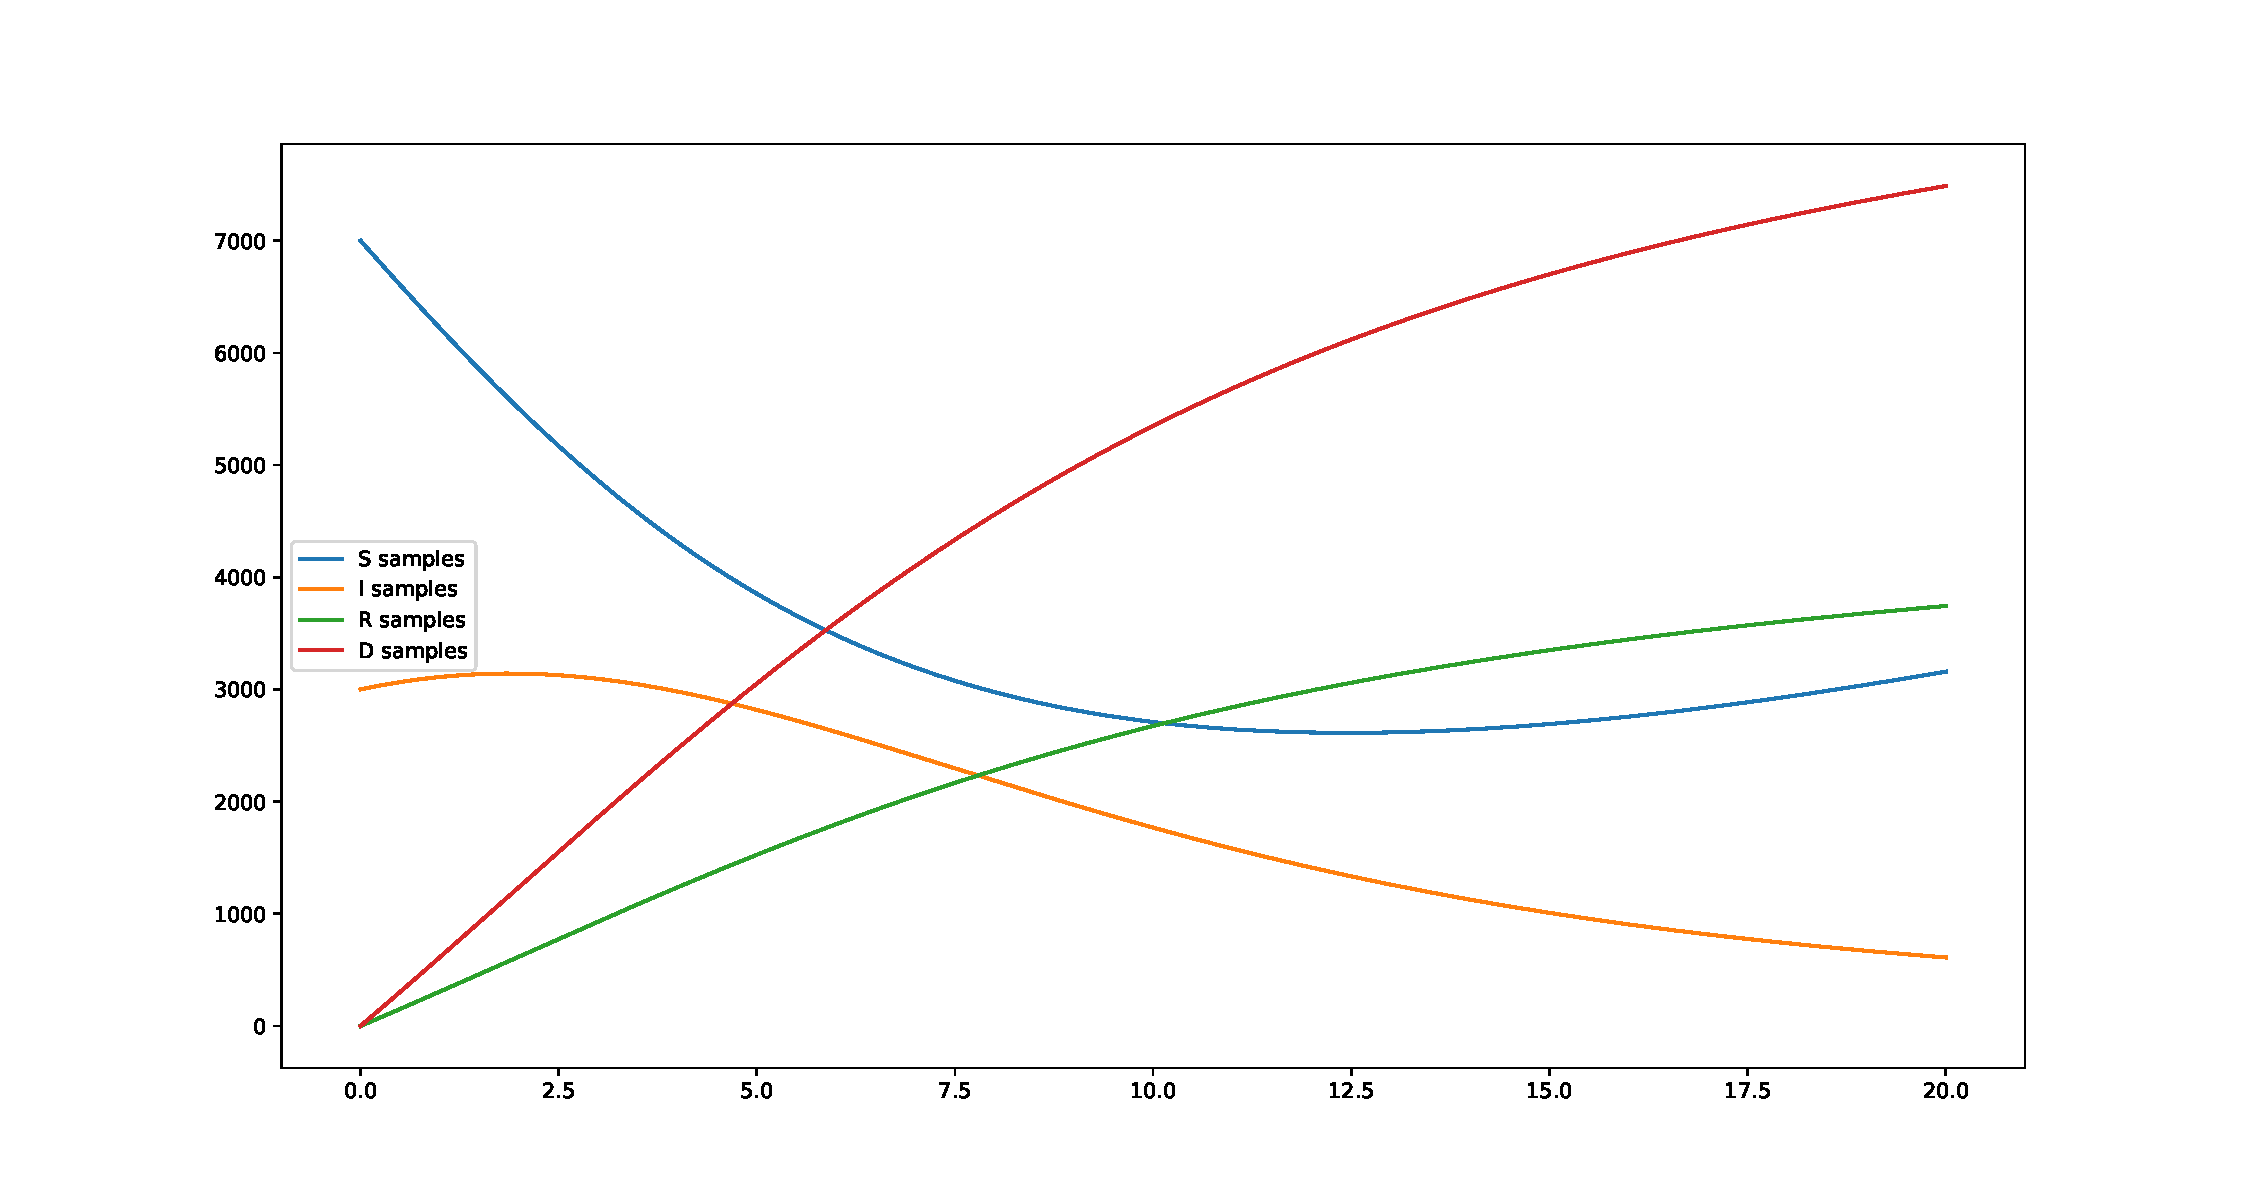
\includegraphics[width=\textwidth]{"figures/SIRD.pdf"}
    \caption{modelo SIRD con $a = 250$, $b = 0.5$, $c = 0.1$ y $d = 0.2$.}
    \label{fig:SIRD}
\end{figure}

Los resultados que se obtienen durante las 30 ejecuciones del experimento aparecen en la tabla \ref{table:experiment_SIRD}.

\begin{table}[!h]
    \centering
    \caption{Resultados obtenidos en el modelo SIRD}
    \begin{tabular}{|c|c|c|c|}
        \hline
               & \textbf{ruido de 0\%} & \textbf{ruido de 5\%} & \textbf{ruido de 10\%} \\
        \hline
        media  & 84.34081              & 132.55477             & 63.33746               \\
        \hline
        mínimo & 3.21345               & 9.82461               & 17.13992               \\
        \hline
        máximo & 763.53435             & 661.49225             & 281.56297              \\
        \hline
    \end{tabular}

    \begin{tabular}{|c|c|c|c|c|c|}
        \hline
                             & \textbf{ruido de 0\%} & \textbf{ruido de 5\%} & \textbf{ruido de 10\%} \\
        \hline
        cantidad de sistemas & 21                    & 17                    & 22                     \\
        \hline
        original             & 478.47017             & 848.56429             & 967.76246              \\
        \hline
        original con ruido   & 478.47017             & 875.75559             & 1030.02565             \\
        \hline
        spline               & 478.47017             & 848.33054             & 965.09632              \\
        \hline
        otro método          & 639.35513             & 604.6624              & 540.61365              \\
        \hline
    \end{tabular}
    \label{table:experiment_SIRD}
\end{table}

Con este experimento se obtiene que los datos evaluados en el sistema generado por la regresión simbólica no se acercan a los datos utilizados para la generación del sistema obtenido en la regresión simbólica. El sistema SIRD utilizado es el único sistema entre todos los experimentos que posee un parámetro solo en una ecuación.

Los datos que se obtienen de la integración del sistema resulante de la regresión simbólica no se asemejan a los datos de la integración del sistema seleccionado para la realización del experimento, la aparición de ruido afecta aún más el ajuste de los datos.

A continuación se muestra el experimento realizado a partir de la generación de datos utilizando el sistema SIQRD.

\subsection{SIQRD}

El modelo SIQRD añade al modelo SIRD la posibilidad de aislamiento de una persona, denotado por $Q$, esto modela la situación en que una persona se aisle para no contagiarse o no contagiar a otros \cite{molter2021mathematical}. Se define el sistema como:

\begin{align*}
    S' & = -\beta (\frac{S I}{S + I + Q + R + D}) - \alpha S + \delta Q \\
    I' & = \beta (\frac{S I}{S + I + Q + R + D}) - \gamma I - \mu I     \\
    Q' & = \alpha S - \delta Q                                          \\
    R' & = \gamma I                                                     \\
    D' & = \mu I,
\end{align*}

donde $\alpha$ indica la relación con que una persona susceptible es enviada a aislamiento, $\beta$ es el índice de transmisión, $\delta$ indica la relación con que una persona en aislamiento social regresa al grupo de susceptibles, $\gamma$ indica el índice de recuperación y $\mu$ el índice de muerte a causa de la enfermedad.

Se utilizaron como valores de los parámetros $\alpha = 0.2$, $\beta = 0.9$, $\delta = 0.1$, $\gamma = 0.1$ y $\mu = 0.05$ con punto inicial $(5000, 3000, 1000, 0, 0)$ y se integró en el intervalo $0 \leq t \leq 20$ para obtener los datos que aparecen en la imagen \ref{fig:SIQRD}. Del conjunto de puntos se seleccionaron 300 muestras como datos para el método de regresión simbólica.

\begin{figure}[h]
    \centering
    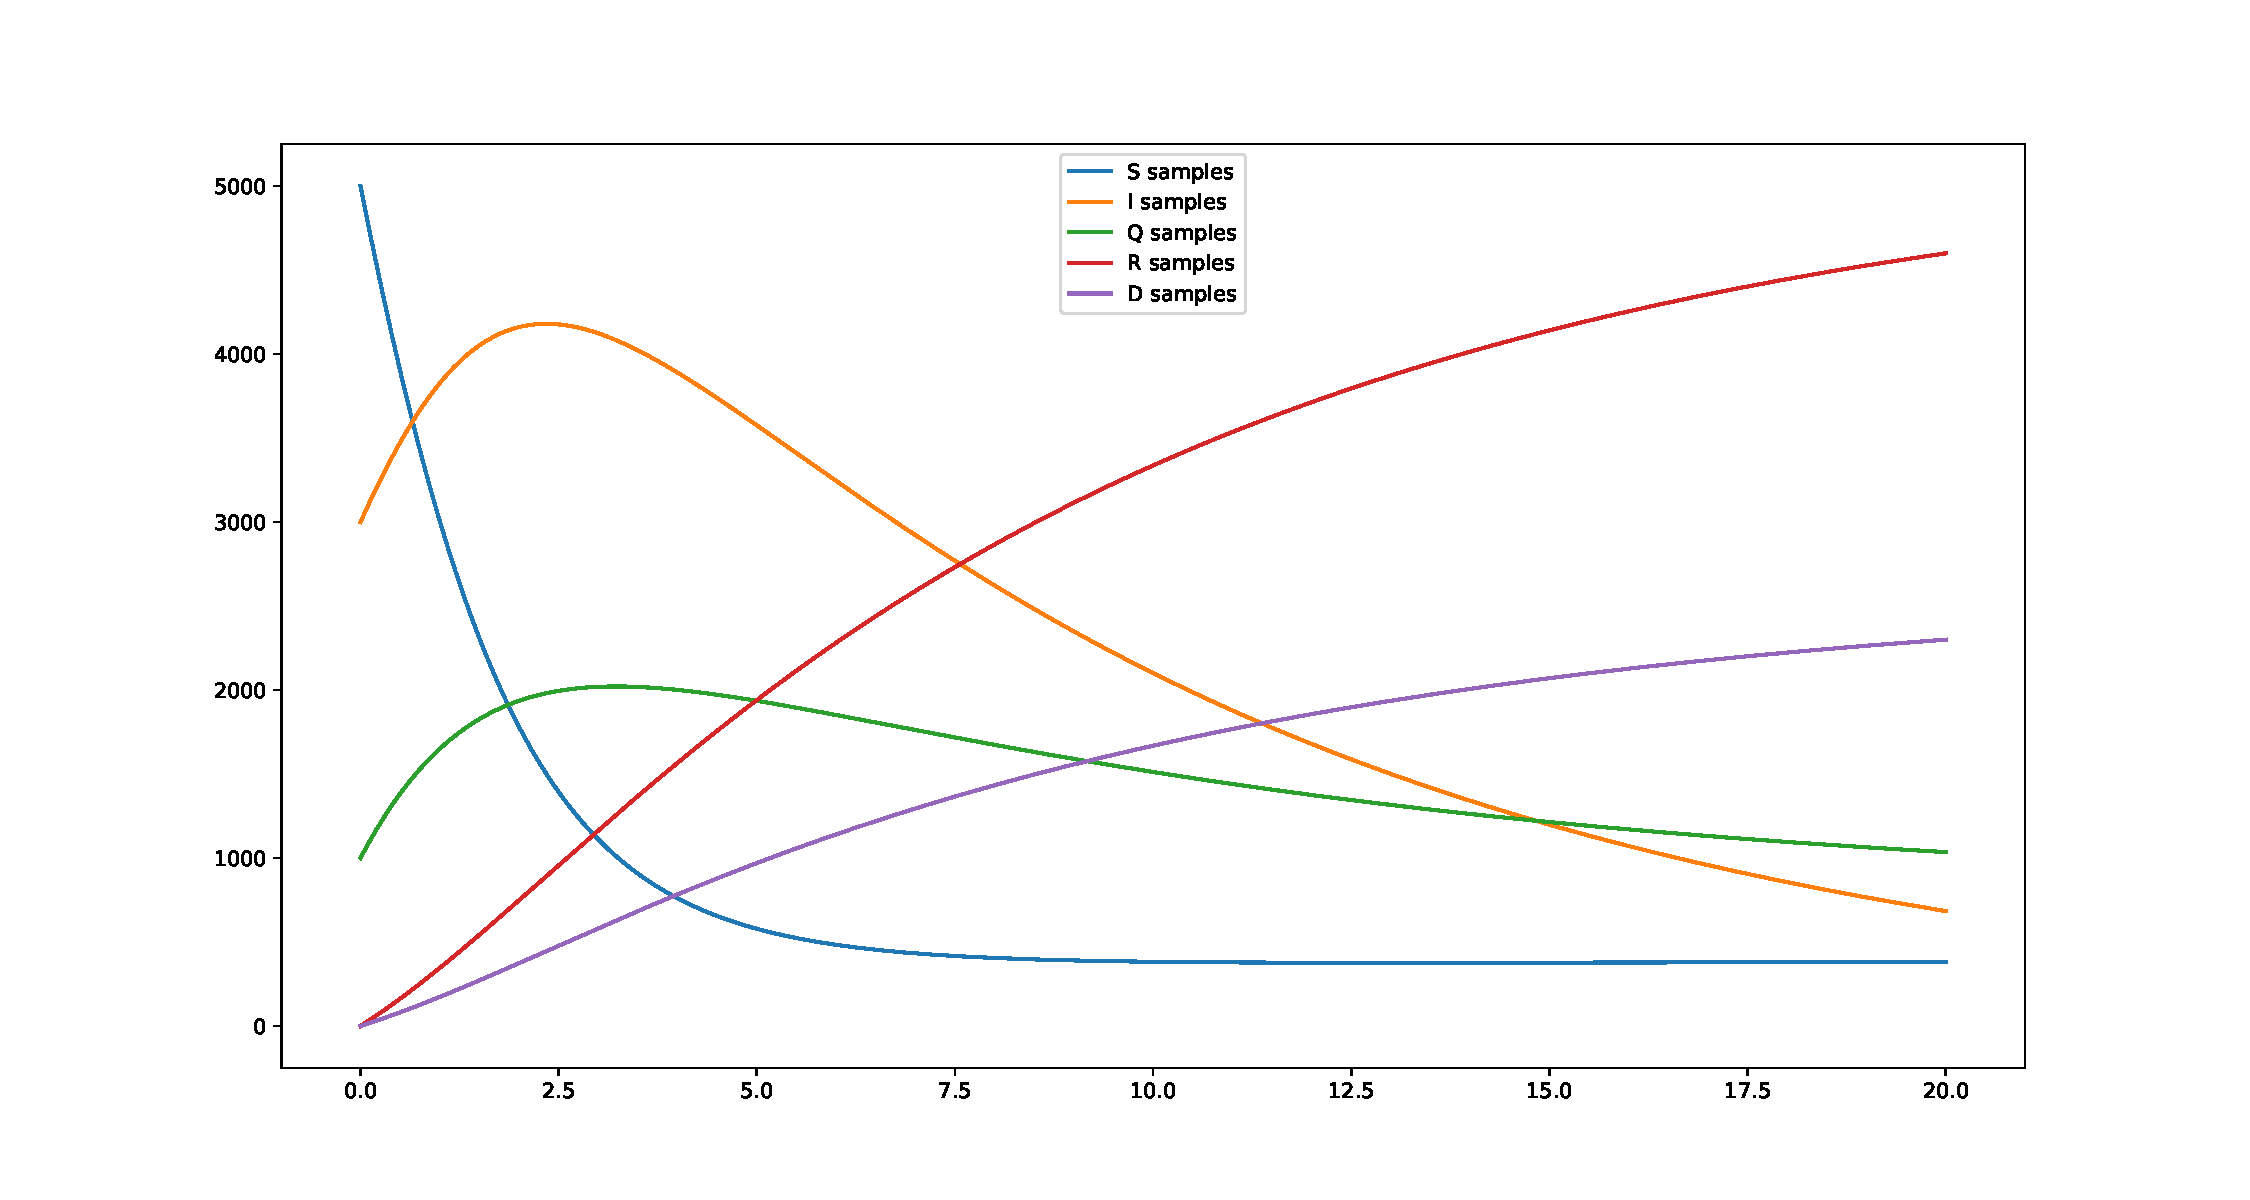
\includegraphics[width=\textwidth]{"figures/SIQRD.pdf"}
    \caption{modelo SIQRD con $\alpha = 0.2$, $\beta = 0.9$, $\delta = 0.1$, $\gamma = 0.1$ y $\mu = 0.05$.}
    \label{fig:SIQRD}
\end{figure}

Los resultados que se obtienen durante las 30 ejecuciones del experimento aparecen en la tabla \ref{table:experiment_SIQRD}.

\begin{table}[!h]
    \centering
    \caption{Resultados obtenidos en el modelo SIQRD}
    \begin{tabular}{|c|c|c|c|}
        \hline
               & \textbf{ruido de 0\%} & \textbf{ruido de 5\%} & \textbf{ruido de 10\%} \\
        \hline
        media  & 7.47098               & 35.17738              & 38.70691               \\
        \hline
        mínimo & 1.35941               & 7.96579               & 12.25428               \\
        \hline
        máximo & 49.24056              & 99.18317              & 197.34403              \\
        \hline
    \end{tabular}

    \begin{tabular}{|c|c|c|c|c|c|}
        \hline
                             & \textbf{ruido de 0\%} & \textbf{ruido de 5\%} & \textbf{ruido de 10\%} \\
        \hline
        cantidad de sistemas & 29                    & 22                    & 22                     \\
        \hline
        original             & 76.49518              & 517.5006              & 338.54534              \\
        \hline
        original con ruido   & 76.49518              & 536.1417              & 395.29378              \\
        \hline
        spline               & 76.49518              & 515.51251             & 338.39969              \\
        \hline
        otro método          & 698.3556              & 919.78558             & 747.2666               \\
        \hline
    \end{tabular}
    \label{table:experiment_SIQRD}
\end{table}

Con este experimento se obtiene que los datos evaluados en el sistema generado por la regresión simbólica se acercan a los datos utilizados para la generación del sistema obtenido en la regresión simbólica mientras los datos utilizados no posean ruido. Los datos que se obtienen de la integración del sistema resulante de la regresión simbólica se asemejan a los datos de la integración del sistema seleccionado para la realización del experimento pero la aparición de ruido afecta el ajuste de los datos. Los datos que se obtienen de la integración del sistema obtenido a partir de un conjunto de datos con ruido máximo de 5\% obtiene peores resultados que si se utiliza como ruido máximo 10\%. Esto se puede deber a un mal ajuste del parámetro de suavizado utilizado en spline de suavizado.

A continuación se muestra el experimento realizado a partir de la generación de datos utilizando el sistema SVVEIR.

\subsection{SVVEIR}

El modelo SVVEIR describe un escenario de una posible enfermedad en la sociedad de Bangladesh. En el modelo se plantea un conjunto $S$ de individuos que no se han infectado aún, $V_1$ y $V_2$ son los individuos que han recibido la primera y segunda vacuna, respectivamente. Las personas infectadas pero que aún no han desarrollado síntomas se definen como expuestos y se encuentran representados por el conjunto $E$. Los parámetros $I$ y $R$ identifican los mismos conjuntos que en el modelo SIR. \cite{kuddus2021mathematical}. Se define el sistema como:


\begin{align*}
    N    & = S + V_1 + V_2 + E + I + R                                        \\
    S'   & = \mu * N - \beta * \frac{I}{N} * S - n * S - \mu * S + \rho * V_1 \\
    V_1' & = n * S - \rho * V_1 - \sigma * V_1 - \mu * V_1                    \\
    V_2' & = \sigma * V_1 - \omega * V_2 - \mu * V_2                          \\
    E'   & = \beta * I / N * S - \alpha * E - \mu * E                         \\
    I'   & = \alpha * E - \gamma * I - \delta * I - \mu * I                   \\
    R'   & = \gamma * I + \omega * V_2 - \mu * R,
\end{align*}

donde $\alpha$ indica la relación de personas expuestas que pasan a estar infectados, $\beta$ es el índice de transmisión de la enfermedad, $\delta$ es índice de muerte debido a la enfermedad mientras que $\mu$ es el índice de muerte por causas naturales. El índice de recuperación de la enfermedad se representa mediante el parámetro $\gamma$. El parámetro $n$ muestra el índice de personas susceptibles que reciben la primera dosis de la vacuna y $\rho$ describe la relación de personas con una sola dosis de la vacuna que regresas al grupo de susceptibles. La cantidad de personas que reciben la segunda dosis se refleja en el parámetro $\sigma$ y $\omega$ es el parámetro que muestra la relación de personas con dos dosis de la vacuna que pasan a recuperados.

Se utilizaron como valores de los parámetros $\alpha = 0.1$, $\beta = 0.7$, $\delta = 0.0005$, $\gamma = 0.05$, $\mu = 0.01$, $n = 0.2$, $\rho = 0.01$, $\omega = 0.05$ y $\sigma = 0.2$ con punto inicial $(5000, 1000, 0, 2000, 1000, 500)$ y se integró en el intervalo $0 \leq t \leq 20$ para obtener los datos que aparecen en la figura \ref{fig:SVVEIR}. Del conjunto de puntos se seleccionaron 300 muestras como datos para el método de regresión simbólica.

\begin{figure}[h]
    \centering
    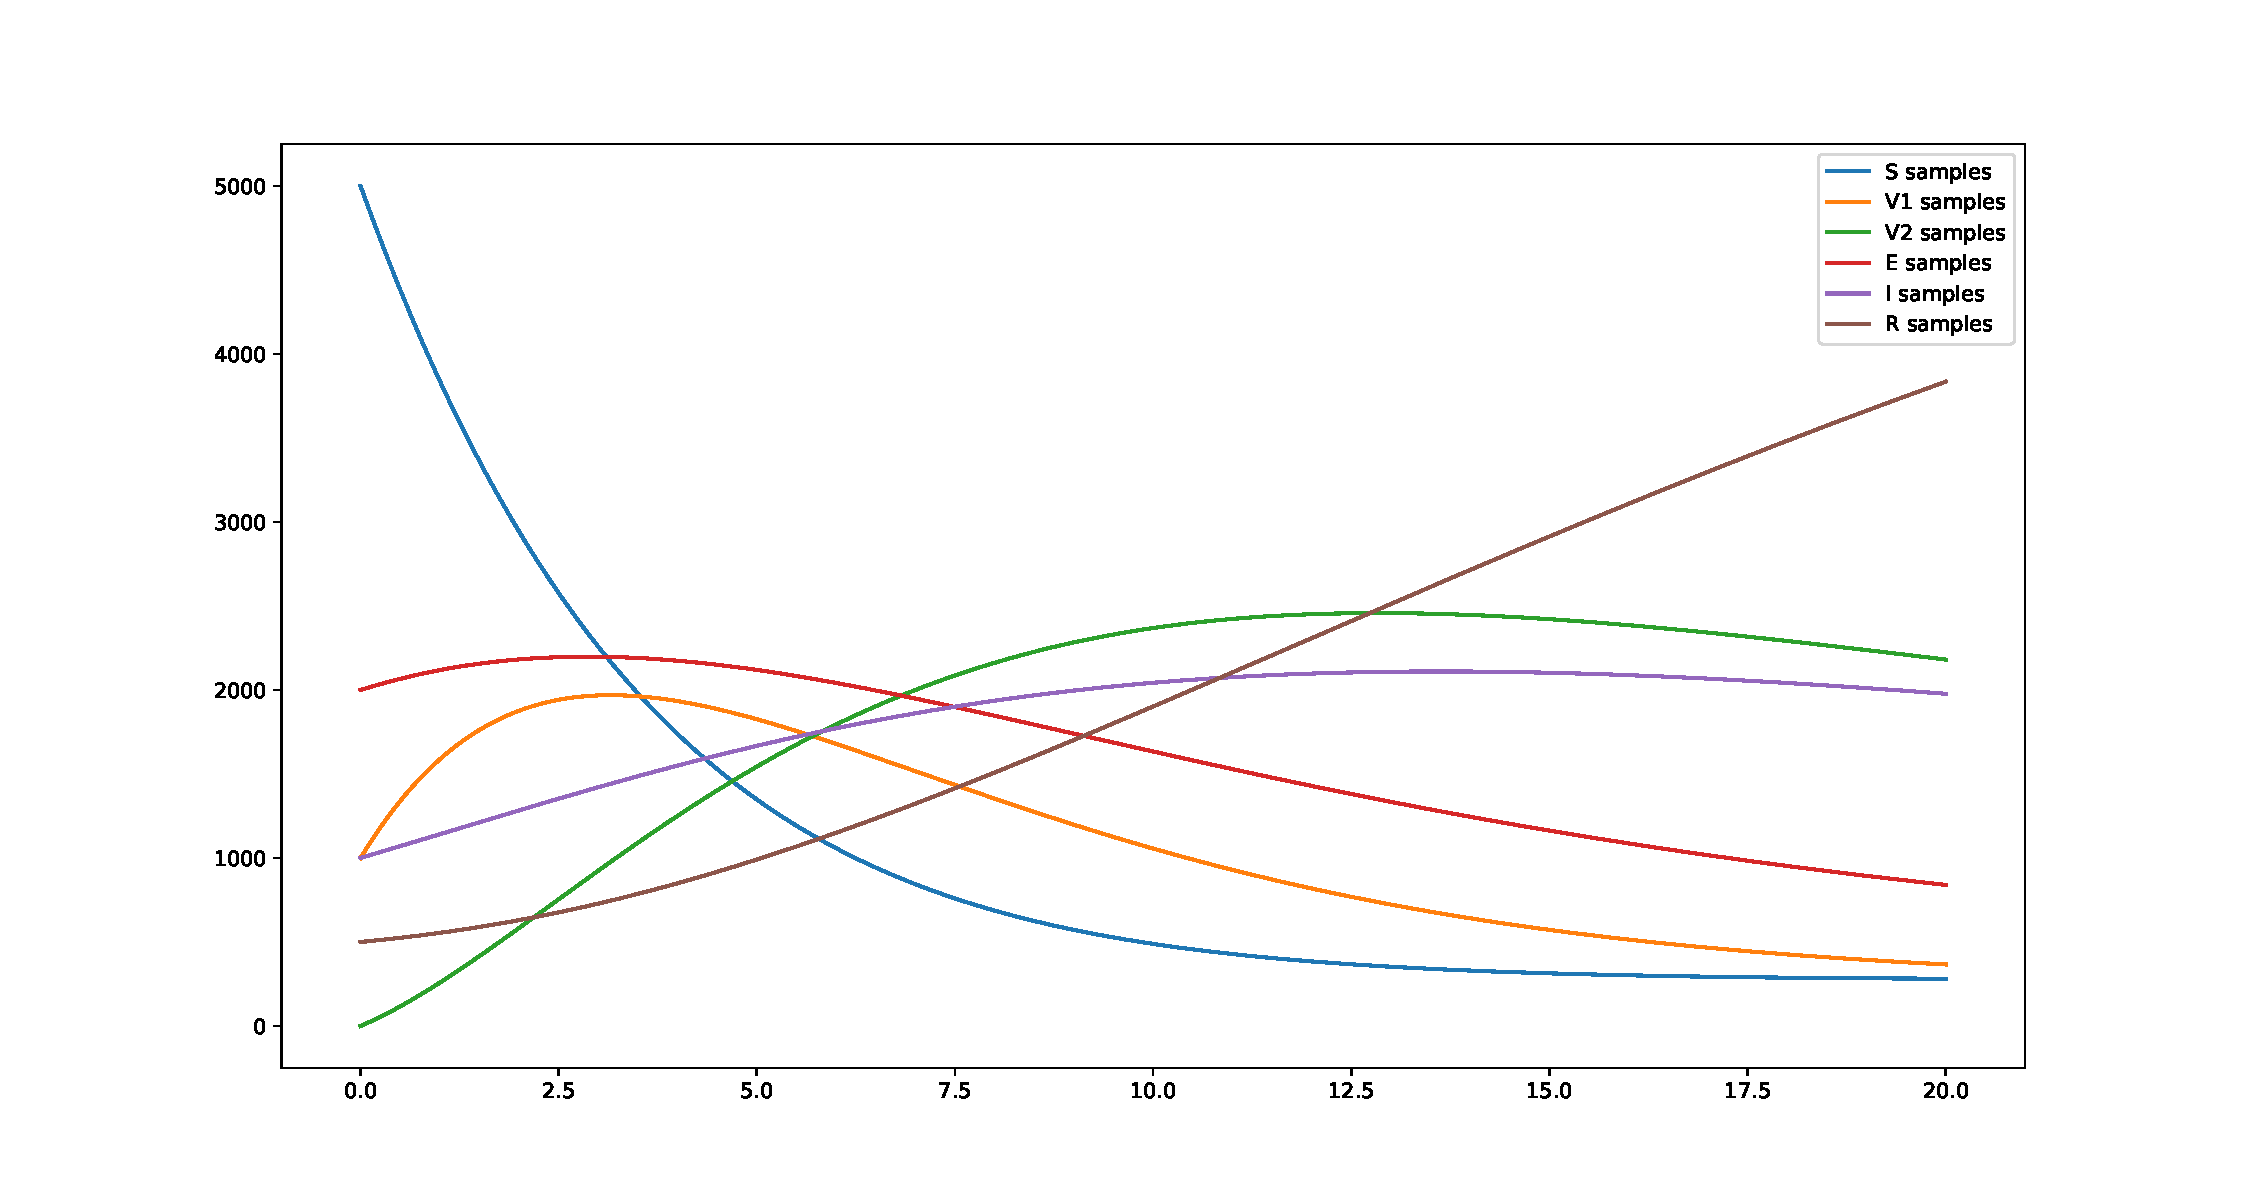
\includegraphics[width=\textwidth]{"figures/SVVEIR.pdf"}
    \caption{modelo SVVEIR con $\alpha = 0.1$, $\beta = 0.7$, $\delta = 0.0005$, $\gamma = 0.05$, $\mu = 0.01$, $n = 0.2$, $\rho = 0.01$, $\omega = 0.05$ y $\sigma = 0.2$.}
    \label{fig:SVVEIR}
\end{figure}

Los resultados que se obtienen durante las 30 ejecuciones del experimento aparecen en la tabla \ref{table:experiment_SVVEIR}.

\begin{table}[!h]
    \centering
    \caption{Resultados obtenidos en el modelo SVVEIR}
    \begin{tabular}{|c|c|c|c|}
        \hline
               & \textbf{ruido de 0\%} & \textbf{ruido de 5\%} & \textbf{ruido de 10\%} \\
        \hline
        media  & 3.64426               & 13.57802              & 16.12164               \\
        \hline
        mínimo & 1.30096               & 9.50931               & 12.69225               \\
        \hline
        máximo & 14.28797              & 29.02875              & 25.4523                \\
        \hline
    \end{tabular}

    \begin{tabular}{|c|c|c|c|c|c|}
        \hline
                             & \textbf{ruido de 0\%} & \textbf{ruido de 5\%} & \textbf{ruido de 10\%} \\
        \hline
        cantidad de sistemas & 30                    & 30                    & 29                     \\
        \hline
        original             & 26.41261              & 121.61259             & 94.25209               \\
        \hline
        original con ruido   & 26.41261              & 146.93245             & 165.1642               \\
        \hline
        spline               & 26.41261              & 121.72339             & 94.75343               \\
        \hline
        otro método          & 1431.78292            & 1415.93366            & 1612.23507             \\
        \hline
    \end{tabular}
    \label{table:experiment_SVVEIR}
\end{table}

Con este experimento se obtiene que los datos evaluados en el sistema generado por la regresión simbólica se acercan a los datos utilizados para la generación del sistema obtenido en la regresión simbólica mientras los datos utilizados no posean ruido. Los datos que se obtienen de la integración del sistema resulante de la regresión simbólica se asemejan a los datos de la integración del sistema seleccionado para la realización del experimento pero la aparición de ruido afecta el ajuste de los datos.

En la siguiente sección se realiza un análisis de los resultados de todos los experimentos realizado.

\section{Análisis de resultados}\label{section:experiments_results}

Los resultados obtenidos durante los experimentos muestran que la regresión simbólica planteada puede encontrar un sistema $f_{aprox}$ que ajuste los datos $y'_{original}$ generados a partir de la derivada aproximada por el método de diferencias finitas sobre los datos $y_{original}$ donde $y_{original}$ son los datos obtenidos de la integración del sistema conocido $f$.

Al generar el conjunto $y_{noise}$ a partir de agregar ruido a $y_{original}$ que describen la función $y$, no se puede aproximar la derivada de $y$ por el método de diferencias finitas. La función $y$ se aproxima utilizando un spline de suavizado cúbico sobre $y_{noise}$ obteniéndose los datos $y_{spline}$. Del spline de suavizado se puede obtener el valor de la primera derivada y así generar el conjunto $y'_{spline}$. Al utilizar los valores de $y_{spline}$ y $y'_{spline}$ en el método de regresión simbólica se obtiene el sistema $f_{aprox_{sr}}$.

El error cuádratico médio de los datos $y_{spline}$ evaluados en el sistema $f_{aprox_{sr}}$ es mayor que el de los datos $y_{original}$ evaluados en el sistema $f_{aprox}$. Mientras mayor el ruido presente en $y_{noise}$ mayor es la diferencia entre los valore del ajuste.

Si se integra el sistema $f_{aprox}$ se obtiene el conjunto de puntos $y_{aprox}$. El valor del error cuádratico medio entre los conjuntos $y_{aprox}$ y $y_{original}$ es menor en los sistemas que no poseen parámetros solos como un sumando en una ecuación.

Si se definen los datos $y_{aprox_{sr}}$ como el resultado de la integración del sistema $f_{aprox_{sr}}$, se puede analizar como el error cuadrático medio entre los puntos $y_{aprox_{sr}}$ y $y_{spline}$ es igual que el error entre los puntos $y_{aprox_{sr}}$ y $y_{original}$.